
%% Sound Questions used on the
%% NYSED Physics Regents Examination
%%--------------------------------------------------

%% this section contains 42 problems

%% Learning Objectives
%%--------------------------------------------------

%% Can recognize that sound behaves as waves


%% Section June2015
%%--------------------
\element{nysed}{
\begin{question}{June2015-Q20}
    The amplitude of a sound wave is most closely related to the sound's:
    \begin{multicols}{2}
    \begin{choices}
        \wrongchoice{speed}
        \wrongchoice{wavelength}
      \correctchoice{loudness}
        \wrongchoice{pitch}
    \end{choices}
    \end{multicols}
\end{question}
}

\element{nysed}{
\begin{question}{June2015-Q28}
    A student listens to music from a speaker in an adjoining room,
        as represented in the diagram below.
    \begin{center}
    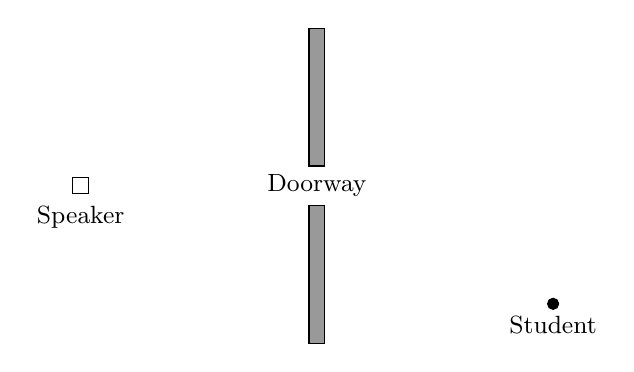
\begin{tikzpicture}[font=\small]
        %% Speaker
        \draw (-3.1,-0.1) rectangle (-2.9,0.1);
        \node[anchor=north,yshift=-1pt] at (-3,-0.1) {Speaker};
        %% Barrier
        \draw[fill=black!40!white] (-0.1,0.25) rectangle (0.1,2);
        \draw[fill=black!40!white] (-0.1,-0.25) rectangle (0.1,-2);
        \node[anchor=center] at (0,0) {Doorway};
        %% Student
        \draw[fill] (3,-1.5) circle (2pt);
        \node[anchor=north,yshift=-1pt] at (3,-1.5) {Student};
    \end{tikzpicture}
    \end{center}
    She notices that she does not have to be directly in front of the doorway to hear the music.
    This spreading of sound waves beyond the doorway is an example of:
    \begin{multicols}{2}
    \begin{choices}
        \wrongchoice{the Doppler effect}
        \wrongchoice{resonance}
        \wrongchoice{refraction}
      \correctchoice{diffraction}
    \end{choices}
    \end{multicols}
\end{question}
}

\element{nysed}{
\begin{question}{June2015-Q32}
    The horn of a moving vehicle produces a sound of constant frequency. 
    Two stationary observers, $A$ and $C$,
        and the vehicle's driver, $B$,
        positioned as represented in the diagram below, hear the sound of the horn.
    \begin{center}
        %% NOTE: insert graphic
        %\includegraphics[width=0.9\columnwidth,keepaspectratio]{June2015-Q32}
    \end{center}
    Compared to the frequency of the sound of the horn heard by driver $B$,
        the frequency heard by observer $A$ is:
    \begin{choices}
        \wrongchoice{lower and the frequency heard by observer $C$ is lower}
        \wrongchoice{lower and the frequency heard by observer $C$ is higher}
        \wrongchoice{higher and the frequency heard by observer $C$ is lower}
        \wrongchoice{higher and the frequency heard by observer $C$ is higher}
    \end{choices}
\end{question}
}


%% Section June2014
%%--------------------
\element{nysed}{
\begin{question}{June2014-Q21}
    What is the period of a sound wave having frequency of \SI{340}{\hertz}?
    \begin{multicols}{2}
    \begin{choices}
      \correctchoice{\SI{2.94e-3}{\second}}
        \wrongchoice{\SI{9.73e-1}{\second}}
        \wrongchoice{\SI{3.40e2}{\second}}
        \wrongchoice{\SI{1.02e2}{\second}}
    \end{choices}
    \end{multicols}
\end{question}
}

\element{nysed}{
\begin{question}{June2014-Q26}
    As a car approaches a pedestrian crossing the road,
        the driver blows the horn.
    Compared to the sound wave emitted by the horn,
        the sound wave detected by the pedestrian has a:
    \begin{choices}
      \correctchoice{higher frequency and a higher pitch}
        \wrongchoice{higher frequency and a lower pitch}
        \wrongchoice{lower frequency and a higher pitch}
        \wrongchoice{lower frequency and a lower pitch}
    \end{choices}
\end{question}
}


%% Section June2013
%%--------------------
\element{nysed}{
\begin{question}{June2013-Q18}
    The energy of a sound wave is most closely related to the wave's:
    \begin{multicols}{2}
    \begin{choices}
        \wrongchoice{frequency}
      \correctchoice{amplitude}
        \wrongchoice{wavelength}
        \wrongchoice{speed}
    \end{choices}
    \end{multicols}
\end{question}
}

\element{nysed}{
\begin{question}{June2013-Q19}
    A sound wave traveling eastward through air causes the air molecules to:
    \begin{choices}
      \correctchoice{vibrate east and west}
        \wrongchoice{vibrate north and south}
        \wrongchoice{move eastward, only}
        \wrongchoice{move northward, only}
    \end{choices}
\end{question}
}

\element{nysed}{
\begin{question}{June2013-Q26}
    Sound waves are produced by the horn of a truck that is approaching a stationary observer.
    Compared to the sound waves detected by the driver of the truck,
        the sound waves detected by the observer have a greater
    \begin{multicols}{2}
    \begin{choices}
        \wrongchoice{wavelength}
        \wrongchoice{period}
      \correctchoice{frequency}
        \wrongchoice{speed}
    \end{choices}
    \end{multicols}
\end{question}
}


%% Section June2012
%%--------------------
\element{nysed}{
\begin{question}{June2012-Q24}
    A tuning fork vibrates at a frequency of \SI{512}{\hertz} when struck with a rubber hammer.
    The sound produced by the tuning fork will travel through the air as a:
    \begin{choices}
      \correctchoice{longitudinal wave with air molecules vibrating parallel to the direction of travel}
        \wrongchoice{transverse wave with air molecules vibrating parallel to the direction of travel}
        \wrongchoice{longitudinal wave with air molecules vibrating perpendicular to the direction of travel}
        \wrongchoice{transverse wave with air molecules vibrating perpendicular to the direction of travel}
    \end{choices}
\end{question}
}

\element{nysed}{
\begin{question}{June2012-Q31}
    What is the wavelength of a \SI{2.50}{\kilo\hertz} sound wave traveling at \SI{326}{\meter\per\second} through air?
    \begin{multicols}{2}
    \begin{choices}
      \correctchoice{\SI{0.130}{\meter}}
        \wrongchoice{\SI{1.30}{\meter}}
        \wrongchoice{\SI{7.67}{\meter}}
        \wrongchoice{\SI{130}{\meter}}
    \end{choices}
    \end{multicols}
\end{question}
}

\element{nysed}{
\begin{question}{June2012-Q33}
    In the diagram below, a stationary source located at point $S$ produces sound having a constant frequency of \SI{512}{\hertz}.
    Observer $A$, \SI{50}{\meter} to the left of $S$, hears a frequency of \SI{512}{\hertz}.
    Observer $B$, \SI{100}{\meter} to the right of $S$, hears a frequency lower than \SI{512}{\hertz}
    \begin{center}
    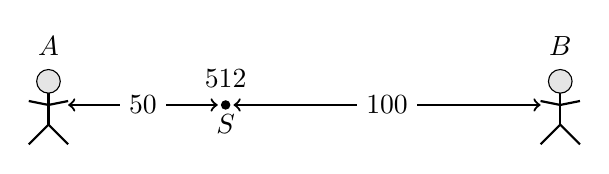
\begin{tikzpicture}
        %% Source
        \draw[fill] (0,0) circle (1.5pt) node[anchor=north] {$S$};
        \node[anchor=south] at (0,0.1) {\SI{512}{\hertz}};
        %% distances
        \draw[thick,<->] (-0.1,0) -- (-2,0) node[pos=0.5,anchor=center,fill=white] {\SI{50}{\meter}};
        \draw[thick,<->] (+0.1,0) -- (4,0) node[pos=0.5,anchor=center,fill=white] {\SI{100}{\meter}};
        %% Labels
        \node[anchor=south] at (-2.25,0.5) {$A$};
        \node[anchor=south] at (+4.25,0.5) {$B$};
        %% Man
        \foreach \x in {-2.25,4.25} {
            \begin{scope}[anchor=south,shift={(\x,-0.5)}]
                \draw[thick] (0,0.25) -- (0,0.75);
                %% Legs
                \draw[thick] (0,0.25) -- (-0.25,0);
                \draw[thick] (0,0.25) -- (+0.25,0);
                %% Arms
                \draw[thick] (0,0.50) -- (-0.25,0.55);
                \draw[thick] (0,0.50) -- (+0.25,0.55);
                %% Head
                \draw[fill=white!90!black] (0,0.80) circle (0.15cm);
            \end{scope}
        }
    \end{tikzpicture}
    \end{center}
    Which statement best describes the motion of the observers?
    \begin{choices}
        \wrongchoice{Observer $A$ is moving toward point $S$, and observer $B$ is stationary.}
        \wrongchoice{Observer $A$ is moving away from point $S$, and observer $B$ is stationary.}
        \wrongchoice{Observer $A$ is stationary, and observer $B$ is moving toward point $S$.}
      \correctchoice{Observer $A$ is stationary, and observer $B$ is moving away from point $S$.}
    \end{choices}
\end{question}
}


%% Section June2011
%%--------------------
\element{nysed}{
\begin{question}{June2011-Q29}
    What is the wavelength of a \SI{256}{\hertz}
        sound wave in air at standard temperature and pressure (STP)?
    \begin{multicols}{2}
    \begin{choices}
        \wrongchoice{\SI{1.17e6}{\meter}}
        \wrongchoice{\SI{0.773}{\meter}}
      \correctchoice{\SI{1.29}{\meter}}
        \wrongchoice{\SI{8.53e-7}{\meter}}
    \end{choices}
    \end{multicols}
\end{question}
}

\element{nysed}{
\begin{question}{June2011-Q31}
    Which statement correctly describes one characteristic of a sound wave?
    \begin{choices}
        \wrongchoice{A sound wave can travel through a vacuum.}
        \wrongchoice{A sound wave is a transverse wave.}
      \correctchoice{The amount of energy a sound wave transmits is directly related to the wave's amplitude.}
        \wrongchoice{The amount of energy a sound wave transmits is inversely related to the wave's frequency.}
    \end{choices}
\end{question}
}


%% Section June2010
%%--------------------


%% Section June2009
%%--------------------
\element{nysed}{
\begin{question}{June2009-Q26}
    The sound wave produced by a trumpet has a frequency of \SI{440}{\hertz}.
    What is the distance between successive compressions in this sound wave as it travels through air at standard temperature and pressure?
    \begin{multicols}{2}
    \begin{choices}
        \wrongchoice{\SI{1.5e-6}{\meter}}
      \correctchoice{\SI{0.75}{\meter}}
        \wrongchoice{\SI{1.3}{\meter}}
        \wrongchoice{\SI{6.8e5}{\meter}}
    \end{choices}
    \end{multicols}
\end{question}
}


%% Section Jan2009
%%--------------------
\element{nysed}{
\begin{question}{Jan2009-Q32}
    A car's horn produces a sound wave of constant frequency.
    As the car speeds up going away from a stationary spectator,
        the sound wave detected by the spectator:
    \begin{choices}
      \correctchoice{decreases in amplitude and decreases in frequency.}
        \wrongchoice{decreases in amplitude and increases in frequency.}
        \wrongchoice{increases in amplitude and decreases in frequency.}
        \wrongchoice{increases in amplitude and increases in frequency.}
    \end{choices}
\end{question}
}


%% Section June2008
%%--------------------
\element{nysed}{
\begin{question}{June2008-Q32}
    A car's horn is producing a sound wave having a constant frequency of \SI{350}{\hertz}.
    If the car moves toward a stationary observer at constant speed,
        the frequency of the car's horn detected by this observer may be:
    \begin{multicols}{2}
    \begin{choices}
        \wrongchoice{\SI{320}{\hertz}}
        \wrongchoice{\SI{350}{\hertz}}
        \wrongchoice{\SI{330}{\hertz}}
      \correctchoice{\SI{380}{\hertz}}
    \end{choices}
    \end{multicols}
\end{question}
}


%% Section Jan2008
%%--------------------
\element{nysed}{
\begin{question}{Jan2008-Q23}
    Increasing the amplitude of a sound wave produced a sound with more:
    \begin{choices}
        \wrongchoice{lower speed}
        \wrongchoice{higher pitch}
        \wrongchoice{shorter wavelength}
      \correctchoice{greater loudness}
    \end{choices}
\end{question}
}

\element{nysed}{
\begin{question}{Jan2008-Q32}
    A police car traveling at a speed of \SI{30.0}{\meter\per\second} sounds its siren,
        which has a frequency of \SI{1.00e3}{\hertz}.
    As the police car approaches a stationary pedestrian,
        the pedestrian detects a siren frequency of:
    \begin{multicols}{2}
    \begin{choices}
        \wrongchoice{\SI{30.0}{\hertz}}
        \wrongchoice{\SI{9.19e2}{\hertz}}
        \wrongchoice{\SI{1.00e3}{\hertz}}
      \correctchoice{\SI{1.10e3}{\hertz}}
    \end{choices}
    \end{multicols}
\end{question}
}

\element{nysed}{
\begin{question}{Jan2008-Q47}
    A sound wave has a wavelength of \SI{5.5}{\meter} as it travels through air at standard temperature and pressure.
    What is the wavelength of this sound in a medium where its speed is \SI{1324}{\meter\per\second}?
    \begin{multicols}{2}
    \begin{choices}
        \wrongchoice{\SI{1.4}{\meter}}
        \wrongchoice{\SI{2.2}{\meter}}
        \wrongchoice{\SI{14}{\meter}}
      \correctchoice{\SI{22}{\meter}}
    \end{choices}
    \end{multicols}
\end{question}
}



%% Section June2007
%%--------------------
\element{nysed}{
\begin{question}{June2007-Q31}
    A student sees a train that is moving away from her and sounding its whistle at a constant frequency.
    Compared to the sound produced by the whistle,
        the sound observed by the student is:
    \begin{choices}
      \correctchoice{lower in pitch}
        \wrongchoice{higher in pitch}
        \wrongchoice{a transverse wave rather than a longitudinal wave}
        \wrongchoice{greater in amplitude}
    \end{choices}
\end{question}
}

\element{nysed}{
\begin{question}{June2007-Q25}
    At an outdoor physics demonstration, a delay of \SI{0.50}{\second} was observed between the time sound waves left a loudspeaker and the time these sound waves reached a student through the air.
    If the air is at standard temperature and pressure,
        how far was the student from the speaker?
    \begin{multicols}{2}
    \begin{choices}
      \correctchoice{\SI{1.7e2}{\meter}}
        \wrongchoice{\SI{1.5e-3}{\meter}}
        \wrongchoice{\SI{6.6e2}{\meter}}
        \wrongchoice{\SI{1.5e8}{\meter}}
    \end{choices}
    \end{multicols}
\end{question}
}



%% Section Jan2007
%%--------------------


%% Section June2006
%%--------------------
\element{nysed}{
\begin{question}{June2006-Q25}
    The energy of a sound wave is most closely related to its:
    \begin{multicols}{2}
    \begin{choices}
      \correctchoice{amplitude}
        \wrongchoice{period}
        \wrongchoice{frequency}
        \wrongchoice{wavelength}
    \end{choices}
    \end{multicols}
\end{question}
}

\element{nysed}{
\begin{question}{June2006-Q26}
    A person observes a fireworks display from a safe distance of \SI{0.750}{\kilo\meter}.
    Assuming that sound travels at \SI{340}{\meter\per\second} in air,
        what is the time between the person seeing and hearing a fireworks explosion?
    \begin{multicols}{2}
    \begin{choices}
      \correctchoice{\SI{2.21}{\second}}
        \wrongchoice{\SI{0.453}{\second}}
        \wrongchoice{\SI{410}{\second}}
        \wrongchoice{\SI{2.55e5}{\second}}
    \end{choices}
    \end{multicols}
\end{question}
}

\element{nysed}{
\begin{question}{June2006-Q48}
    A \SI{512}{\hertz} sound wave travels \SI{100}{\meter} to an observer through air at standard temperature and pressure.
    What is the wavelength of this sound wave?
    \begin{multicols}{2}
    \begin{choices}
      \correctchoice{\SI{0.646}{\meter}}
        \wrongchoice{\SI{0.195}{\meter}}
        \wrongchoice{\SI{1.55}{\meter}}
        \wrongchoice{\SI{5.12}{\meter}}
    \end{choices}
    \end{multicols}
\end{question}
}




%% Section Jan2006
%%--------------------


%% Section June2005
%%--------------------


%% Section Jan2005
%%--------------------
\element{nysed}{
\begin{question}{Jan2005-Q19}
    A train sounds a whistle of constant frequency as it leaves the train station.
    Compared to the sound emitted by the whistle,
        the sound that the passengers standing on the platform hear has a frequency that is:
    \begin{choices}
      \correctchoice{lower, because the sound-wave fronts reach the platform at a frequency lower than the frequency at which they are produced}
        \wrongchoice{lower, because the sound waves travel more slowly in the still air above the platform than in the rushing air near the station.}
        \wrongchoice{higher, because the sound-wave fronts reach the platform at a frequency higher than the frequency at which they are produced.}
        \wrongchoice{higher, because the sound waves travel faster in the still air above the platform than in the rushing air near the station.}
    \end{choices}
\end{question}
}

\element{nysed}{
\begin{question}{Jan2005-Q13}
    A tuning fork vibrating in air produces sound waves.
    These waves are best classified as:
    \begin{choices}
      \correctchoice{longitudinal, because the air molecules are vibrating parallel to the direction of wave motion.}
        \wrongchoice{longitudinal, because the air molecules are vibrating perpendicular to the direction of wave motion.}
        \wrongchoice{transverse, because the air molecules are vibrating parallel to the direction of wave motion.}
        \wrongchoice{transverse, because the air molecules are vibrating perpendicular to the direction of wave motion.}
    \end{choices}
\end{question}
}



%% Section June2004
%%--------------------
\element{nysed}{
\begin{question}{June2004-Q28}
    As a sound wave passes from water,
        where the speed is \SI{1.49e3}{\meter\per\second}, into air, the wave's speed:
    \begin{choices}
      \correctchoice{decreases and its frequency remains the same}
        \wrongchoice{increases and its frequency remains the same}
        \wrongchoice{remains the same and its frequency decreases}
        \wrongchoice{remains the same and its frequency increases}
    \end{choices}
\end{question}
}

\element{nysed}{
\begin{question}{June2004-Q27}
    An electric bell connected to a battery is sealed inside a large jar.
    What happens as the air is removed from the jar?
    \begin{choices}
      \correctchoice{The bell's loudness decreases because sound waves can \emph{not} travel through a vacuum}
        \wrongchoice{The electric circuit stops working because electromagnetic radiation can \emph{not} travel through a vacuum}
        \wrongchoice{The bell's pitch decreases because the frequency of the sound waves is lower in a vacuum than in air}
        \wrongchoice{The bell's loudness increases because of decreased air resistance}
    \end{choices}
\end{question}
}


%% Section Jan2004
%%--------------------
\element{nysed}{
\begin{question}{Jan2004-Q29}
    Which wave phenomena makes it possible for a player to hear the sound from a referee's whistle in an open field even when standing behind the referee?
    \begin{multicols}{2}
    \begin{choices}
      \correctchoice{diffraction}
        \wrongchoice{Doppler effect}
        \wrongchoice{reflection}
        \wrongchoice{refraction}
    \end{choices}
    \end{multicols}
\end{question}
}

\element{nysed}{
\begin{question}{Jan2004-Q41}
    A system consists of an oscillator and a speaker that emits a \SI{1000}{\hertz} sound wave.
    A microphone detects the sound wave \SI{1.00}{\meter} from the speaker.
    \begin{center}
        %% NOTE: complex, keep this
        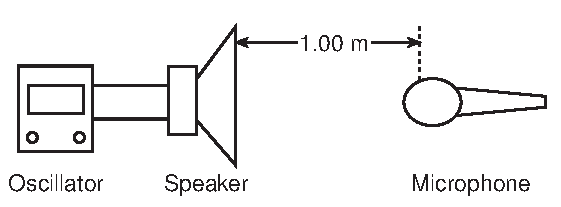
\includegraphics[keepaspectratio,scale=0.75]{Jan2004-Q41}
    \end{center}
    Which type of wave is emitted by the speaker?
    \begin{multicols}{2}
    \begin{choices}
      \correctchoice{longitudinal}
        \wrongchoice{transverse}
        \wrongchoice{circular}
        \wrongchoice{electromagnetic}
    \end{choices}
    \end{multicols}
\end{question}
}

\element{nysed}{
\begin{question}{Jan2004-Q42}
    A system consists of an oscillator and a speaker that emits a \SI{1000}{\hertz} sound wave.
    A microphone detects the sound wave \SI{1.00}{\meter} from the speaker.
    \begin{center}
        %% NOTE: complex, keep this
        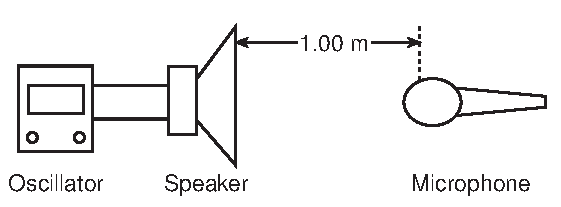
\includegraphics[keepaspectratio,scale=0.75]{Jan2004-Q41}
    \end{center}
    The microphone is moved to a new fixed location \SI{0.50}{\meter} in front of the speaker.
    Compared to the sound waves detected at the \SI{1.00}{\meter} position, the sound waves detected at the \SI{0.50}{\meter} position have a different.
    \begin{multicols}{2}
    \begin{choices}
      \correctchoice{amplitude}
        \wrongchoice{frequency}
        \wrongchoice{wave speed}
        \wrongchoice{wavelength}
    \end{choices}
    \end{multicols}
\end{question}
}

\element{nysed}{
\begin{question}{Jan2004-Q43}
    A system consists of an oscillator and a speaker that emits a \SI{1000}{\hertz} sound wave.
    A microphone detects the sound wave \SI{1.00}{\meter} from the speaker.
    \begin{center}
        %% NOTE: complex, keep this
        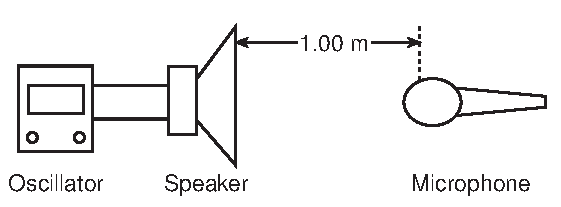
\includegraphics[keepaspectratio,scale=0.75]{Jan2004-Q41}
    \end{center}
    The microphone is moved at constant speed from the \SI{0.50}{\meter} position back to its original position \SI{1.00}{\meter} from the speaker.
    Compared to the \SI{1000}{\hertz} frequency emitted by the speaker,
        the frequency detected by the moving microphone is:
    \begin{multicols}{3}
    \begin{choices}
      \correctchoice{lower}
        \wrongchoice{higher}
        \wrongchoice{the same}
    \end{choices}
    \end{multicols}
\end{question}
}


%% Section June2003
%%--------------------
\element{nysed}{
\begin{question}{June2003-Q30}
    A sound of constant frequency is produce by the siren on top of a firehouse.
    Compared to the frequency produced by the siren,
        the frequency observed by a firefighter approaching the firehouse is:
    \begin{multicols}{3}
    \begin{choices}
      \correctchoice{lower}
        \wrongchoice{higher}
        \wrongchoice{the same}
    \end{choices}
    \end{multicols}
\end{question}
}


%% Section Jan2003
%%--------------------


%% Section Aug2002
%%--------------------
\element{nysed}{
\begin{question}{Aug2002-Q16}
    An electric guitar is generating a sound of constant frequency.
    An increase in which sound wave characteristic would result in an increase in loudness?
    \begin{multicols}{2}
    \begin{choices}
        \wrongchoice{speed}
        \wrongchoice{period}
        \wrongchoice{wavelength}
      \correctchoice{amplitude}
    \end{choices}
    \end{multicols}
\end{question}
}


%% Section June2002
%%--------------------
\element{nysed}{
\begin{question}{June2002-Q29}
    A source of sound waves approaches a stationary observer through a uniform medium.
    Compared to the frequency and wavelength of the emitted sound,
        the observer would detect waves with a:
    \begin{choices}
      \correctchoice{higher frequency and shorter wavelength.}
        \wrongchoice{higher frequency and longer wavelength.}
        \wrongchoice{lower frequency and shorter wavelength.}
        \wrongchoice{lower frequency and longer wavelength.}
    \end{choices}
\end{question}
}


%% Section Jan2002
%%--------------------


%% Section June2001
%%--------------------
\element{nysed}{
\begin{question}{June2001-Q41}
    What type of wave is sound traveling in water?
    \begin{multicols}{2}
    \begin{choices}
        \wrongchoice{torsional}
        \wrongchoice{transverse}
        \wrongchoice{elliptical}
      \correctchoice{longitudinal}
    \end{choices}
    \end{multicols}
\end{question}
}


%% Section Jan2001
%%--------------------
\element{nysed}{
\begin{question}{Jan2001-Q49}
    The driver of a car blows the horn as the car approaches a crosswalk.
    Compared to the actual pitch of the horn,
        the pitch observed by a pedestrian in the crosswalk is:
    \begin{multicols}{3}
    \begin{choices}
        \wrongchoice{lower}
      \correctchoice{higher}
        \wrongchoice{the same}
    \end{choices}
    \end{multicols}
\end{question}
}


%% Section June2000
%%--------------------
\element{nysed}{
\begin{question}{June2000-Q43}
    The diagram below shows a tuning fork vibrating in air.
    The dots represents air molecules as the sound wave moves toward the right.
    \begin{center}
    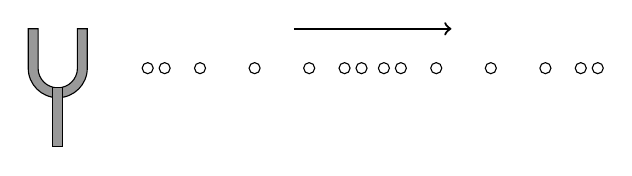
\begin{tikzpicture}
        %% tuning fork
        \begin{scope}[xshift=-1cm,xscale=0.25,yscale=0.25]
            \draw[fill=white!60!black] (-1,2) -- (-1,0) arc (180:360:1) -- (1,2) -- (1.5,2) -- (1.5,0) arc (360:180:1.5) -- (-1.5,2) -- cycle;
            \draw[fill=white!60!black] (-0.25,-1) rectangle (0.25,-4);
        \end{scope}
        %% wave fronts
        \foreach \x in {0,1}
            \foreach \y in {-3,-2,...,3} {
                \draw ({3*\x + (3/(1 + exp(-\y)))},0) circle (2pt);
            }
        %% vector
        \draw[thick,->] (2,0.5) -- (4,0.5);
    \end{tikzpicture}
    \end{center}
    Which diagram best represents the direction of motion of the air molecules?
    \begin{multicols}{2}
    \begin{choices}
        \AMCboxDimensions{down=-0.8cm}
        \wrongchoice{
            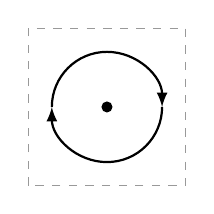
\begin{tikzpicture}[scale=2]
                \draw[dashed,white!60!black] (0,0) rectangle (1,1);
                \fill (0.5,0.5) circle (1pt);
                \draw[thick,-latex] (0.15,0.5) arc (180:0:0.35);
                \draw[thick,-latex] (0.85,0.5) arc (360:180:0.35);
            \end{tikzpicture}
        }
        \wrongchoice{
            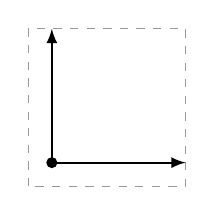
\begin{tikzpicture}[scale=2]
                \draw[dashed,white!60!black] (0,0) rectangle (1,1);
                \fill (0.15,0.15) circle (1pt);
                \draw[thick,-latex] (0.15,0.15) -- (0.15,1);
                \draw[thick,-latex] (0.15,0.15) -- (1,0.15);
            \end{tikzpicture}
        }
        \wrongchoice{
            \begin{tikzpicture}[scale=2]
                \draw[dashed,white!60!black] (0,0) rectangle (1,1);
                \fill (0.5,0.5) circle (1pt);
                \draw[thick,<->] (0.5,1) -- (0.5,0);
            \end{tikzpicture}
        }
        %% ANS is D
        \correctchoice{
            \begin{tikzpicture}[scale=2]
                \draw[dashed,white!60!black] (0,0) rectangle (1,1);
                \fill (0.5,0.5) circle (1pt);
                \draw[thick,<->] (0,0.5) -- (1,0.5);
            \end{tikzpicture}
        }
    \end{choices}
    \end{multicols}
\end{question}
}


%% Section June1999
%%--------------------


%% Section June1998
%%--------------------
\element{nysed}{
\begin{question}{June1998-Q35}
    As a sound wave travels through air,
        there is a net transfer of:
    \begin{choices}
      \correctchoice{energy, only}
        \wrongchoice{mass, only}
        \wrongchoice{both mass and energy}
        \wrongchoice{neither mass nor energy}
    \end{choices}
\end{question}
}


%% Section June1997
%%--------------------
\element{nysed}{
\begin{question}{June1997-Q41}
    The driver of a car sounds the horn while traveling toward a stationary person.
    Compared to the sound heard by the driver,
        the sound heard by the stationary person has:
    \begin{choices}
        \wrongchoice{lower pitch and shorter wavelength}
        \wrongchoice{lower pitch and longer wavelength}
      \correctchoice{higher pitch and shorter wavelength}
        \wrongchoice{higher pitch and longer wavelength}
    \end{choices}
\end{question}
}

\element{nysed}{
\begin{question}{June1997-Q47}
    As shown in the diagram below, speakers $S_1$ and $S_2$,
        separated by a distance of \SI{0.50}{\meter},
        are producing sound of the same frequency.
    A person walking along a path \SI{4.0}{\meter} in front of the speakers hears the sound reach a maximum intensity every \SI{2.0}{\meter}.
    \begin{center}
    \begin{tikzpicture}
        %% NOTE: finish this
    \end{tikzpicture}
    \end{center}
    What is the wavelength of the sound produced by the speakers?
    \begin{multicols}{2}
    \begin{choices}
        \wrongchoice{\SI{1.0}{\meter}}
        \wrongchoice{\SI{0.063}{\meter}}
        \wrongchoice{\SI{0.25}{\meter}}
        \wrongchoice{\SI{4.0}{\meter}}
    \end{choices}
    \end{multicols}
\end{question}
}


%% Section June1996
%%--------------------


%% Section June1995
%%--------------------
\element{nysed}{
\begin{question}{June1995-Q44}
    When an opera singer hits a high pitch note,
        a glass on the opposite side of the opera hall shatters.
    Which statement best explains this phenomenon?
    \begin{choices}
      \correctchoice{The frequency of the note and natural vibration frequency of the glass are equal.}
        \wrongchoice{The vibrations of the note are polarized by the shape of the opera hall.}
        \wrongchoice{The amplitude of the note increases before it reaches the glass.}
        \wrongchoice{The singer and glass are separated by an integral number of wavelengths.}
    \end{choices}
\end{question}
}


%% Section June1994
%%--------------------
\element{nysed}{
\begin{question}{June1994-Q37}
    A characteristic common to sound waves and light waves is that they:
    \begin{multicols}{2}
    \begin{choices}
        \wrongchoice{are longitudinal}
        \wrongchoice{are transverse}
      \correctchoice{transfer energy}
        \wrongchoice{travel in a vacuum}
    \end{choices}
    \end{multicols}
\end{question}
}


%% Section June1986
%%--------------------
\element{nysed}{
\begin{question}{June1986-Q55}
    As the energy imparted to a mechanical wave increases,
        the maximum displacement of the particles in the medium:
    \begin{choices}
        \wrongchoice{decreases}
      \correctchoice{increases}
        \wrongchoice{remains the same}
    \end{choices}
\end{question}
}


%% Section June1985
%%--------------------
\element{nysed}{
\begin{question}{June1985-Q23}
    The driver of a car hears the siren of an ambulance which is moving away from her.
    If the actual frequency of the siren is \SI{2 000}{\hertz},
        the frequency heard by the driver must be:
    \begin{multicols}{2}
    \begin{choices}
      \correctchoice{\SI{1900}{\hertz}}
        \wrongchoice{\SI{2000}{\hertz}}
        \wrongchoice{\SI{1900}{\hertz}}
        \wrongchoice{\SI{4000}{\hertz}}
    \end{choices}
    \end{multicols}
\end{question}
}



\endinput


